\chapter{Характеристика объекта исследования}
\section{Характеристика участка изысканий}
Исследования проводились на образцах, отобранных на участке изысканий под жилой комплекс Саларьево-парк.

Геологический разрез исследуемой территории был изучен на глубину 35,0~м.

Условия их залегания, распространения, состав, состояние зависят от возраста и генезиса и создают довольно разнородную картину. Изучались дисперсные грунты, представленные глинами и суглинками твердой, полутвердой и тугопластичной консистенции.


Геологический разрез на участке представлен разновозрастными отложениями различного генезиса.
Геологический разрез исследуемой территории был изучен на глубину 29,0~м, и представлен следующими стратиграфическими подразделениями:

1) Поверхность исследуемого участка покрыта почвенно-растительным слоем. Во всех скважинах встречены насыпные грунты (t H), представленные суглинком мягкопластичным, перекопанным, с прослоями песка, с включениями обломков бетона, битого кирпича, стекла, остатков древесины. Мощность насыпных грунтов составила 0,2-0,5 м.

2) Верхнечетвертичные покровные отложения (pr III) залегают повсеместно под насыпными грунтами и представлены глинами коричневыми с прослоями и пятнами серых глин, полутвердыми, местами до тугопластичных, с прослоями ожелезнений. Мощность глин составляет 1,6-1,7 м с абс. отм. подошвы 182,8-183,0 м.

3) Среднечетвертичные флювиогляциальные и озерно-ледниковые отложения московского горизонта (f,lg II ms) залегают ниже по разрезу, и представлены переслаивающейся толщей супесей, суглинков и песков. Пески мелкие, светло-коричневые, коричневые, средней плотности, глинистые, с прослоями суглинка и супеси, средней степени водонасыщения. Мощность песков составляет 0,2~м. Супеси светло-коричневые, коричневые, пластичные, слоистые, песчанистые пластичные, вскрыты в подошве флювиогляциальных отложений в виде прослоя мощностью 0,6 м. Суглинки коричневые, светло-коричневые, тугопластичные, пылеватые, слоистые, слагают основную толщу флювиогляциальных отложений в виде слоя мощностью 0,2-1,7 м. Общая мощность флювиогляциальных отложений московского горизонта составляет 1,3-1,7 м с абс. отм. подошвы 181,1-181,7 м.

4) Среднечетвертичные ледниковые отложения московского горизонта (g II ms) залегают под флювиогляциальными отложениями. Они представлены суглинками от коричневых до красновато-коричневых, тугопластичные, местами полутвердые, песчанистые, с прослоями супеси и песка, с включениями дресвы и щебня преимущественно карбонатных пород до 10-15\%. В подошве с прослоями песка мелкого коричневого насыщенного водой. Их мощность колеблется от 0,9 м до 2,1 м с абс. отм. подошвы 179,6-180,3 м.

5) Нижне-среднечетвертичные флювиогляциальные, ледниково-озерные, аллювиальные и озерные отложения донского-московского горизонта (f,lg I-II ds-ms) залегают повсеместно под флювиогляциальными и ледниковыми отложениями московского горизонта. Они представлены суглинками в кровле и в подошве, и глинами в средней части. Суглинки тугопластичные от светло-коричневых до зеленовато-коричнево-серых, тугопластичные, местами до полутвердых, песчанистые, слабо слоистые, с редкими включениями гравия и гальки, залегают преимущественно в кровле и подошве флювиогляциальных отложений. Мощность суглинков колеблется от 1,1 до 3,4 м. Глины серые, темно-серые, с зеленоватым оттенком, полутвердые, в кровле 0,2 м тугопластичные, слоистые, пылеватые, с единичными включениями гравия и гальки, преимущественно залегают в средней части толщи флювиогляциальных отложений донского-московского горизонта, и вскрыты всеми скважинами. Мощность глин составила 2,8-3,8 м. Общая мощность флювиогляциальных отложений донского-московского горизонта составляет 6,7-8,2 м с абсолютной отметкой подошвы 171,6-173,4 м.

6) Ниже залегают нижнечетвертичные ледниковые отложения донского горизонта (g I ds). Они представлены мощной толщей суглинков коричневых, до темно-серо-коричневых, полутвердых, в кровле 0,1-0,3 м тугопластичных, песчанистых, с включениями дресвы и щебня преимущественно карбонатных пород до 15\%. Мощность этих суглинков составила 14,4 м, с абсолютной отметкой подошвы 157,2 м.

7) Завершают разрез на изученную глубину (29,0 м) отложения нижнего отдела меловой системы (K1). Они представлены песками пылеватыми. Пески пылеватые, темно-серые, плотные, глинистые, слюдистые, насыщенные водой. Максимально вскрытая мощность этих песков составила 1,2 м.

Химический состав воды характеризуется как сульфатно-хлоридно-гидрокарбонатный магниево-кальциевый пресный с минерализацией 0,9 г/л, рН равен 7,9. Вода неагрессивная к бетону на портландцементе любых марок, слабоагрессивная к железобетонным конструкциям. Отмечается средняя коррозионная агрессивность к свинцовым и высокая к алюминиевым оболочкам кабелей.


Для испытаний были выбраны образцы четырёх разновидностей: суглинки тугопластичные московского горизонта (ИГЭ № 6), суглинки тугопластичные московско-донского горизонта (ИГЭ № 7), суглинки полутвердые московско-донского горизонта (ИГЭ № 8), ледниковые отложения донского горизонта (ИГЭ № 9). 

Физико-механические свойства, химический и гранулометрический состав были определены в Центральной грунтово-химической лаборатории ООО <<ГеоГрадСтрой>> автором и сотрудниками лаборатории,
часть компрессионых испытаний и минералогический состав был определен рентгенодифракционным анализом в Лаборатории грунтоведения и технической мелиорации грунтов МГУ.

\section{Физические свойства}

Испытания грунтов проводились в соответствии с методами, приведенными в действующих нормативных документах:
плотность $\rho$, 
плотность твердых частиц $\rho_s$, 
влажность $w_e$, 
влажность на границе раскатывания и текучести ($w_L$ и $w_p$) "--- по ГОСТ 5180-2015. 
Рассчитаны такие параметры для глинистых грунтов, как
плотность сухого грунта $\rho_d$,  
коэффициент водонасыщения $S_r$, 
число пластичности $I_p$ 
и показатель текучести $I_L$ по ГОСТ 25100-2011.
%Компрессионые испытания проводились в соответствии с ГОСТ 12248-2010 и ГОСТ 58326-2018.
 

\section{Гранулометрический состав}

Также были проведены определения гранулометрического состава озерно-ледниковых и ледниковых отложений московского и донского горизонта ареометрическим методом. Определение проводилось по ГОСТ 12536-2014. В результате была построена треугольная диаграмма гранулометрического состава (рис.5).

\begin{figure}[ht]
    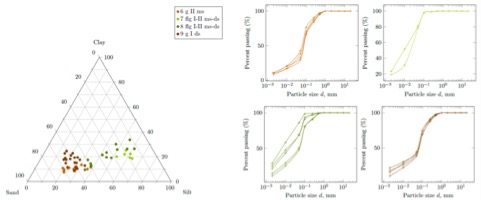
\includegraphics[scale=0.5]{gran.jpg}
    \caption{Результаты гранулометрического анализа: а)"---треугольная диаграмма; б)"---кумулятивные кривые.}
\end{figure}

Гранулометрический состав определялся только для песчанисто-глинистых фракций, без учета крупнообломочной составляющей.
По результатам гранулометрического состава были построены кумулятивные кривые, а также треугольная диаграмма.
Кумулятивные кривые построены в полулогарифическом масштабе, 
по оси абсцисс отложены логарифмы диаметров частиц, 
а по оси ординат накопленное содержание фракции в процентах.

Треугольная диаграмма служит для отправной точкой для некоторых классификаций грунтов, например по В.В. Охотину.
Помимо того, треугольная диаграмма является удобным способом показать большое число результатов и выявить характерные области.

На диаграмме видно, что моренные отложения московского и донского горизонтов образуют довольно кучную группу в области песчанистых суглинков.
Отложения различного генезиса московско-донского горизонта, напротив, более разнообразны по составу, но тяготеют к области 
пылеватых суглинков.

 В соответсвии с вышеперечисленной классификацией В.В. Охотина, 
 6 от супеси тяжелой до суглинка легкого
 7 от суглинка среднего пылеватого до суглинка тяжелого пылеватого
 8 от суглинка легкого до суглинка тяжелого пылеватого
 9 от суглинка легкого до суглинка среднего.

 \section{Минералогический состав} 

В целях дополнительного изучения свойств образцов был сделан рентгено-структурный анализ ледниковых и озерно-ледниковых отложений московского и донского горизонта в лаборатории кафедры инженерной и экологической геологии геологического факультета Московского университета им. М.В. Ломоносова. 




В качестве образцов использовались неориентированные препараты. Растертые предварительно образцы набивались в специальные кюветы без использования прессования при постоянном контроле качества поверхности для приготовления максимально разориентированного препарата.

Рентгенодифракционный анализ порошковых препаратов проводился при помощи рентгеновского дифрактометра ULTIMA-IV фирмы Rigaku (Япония). Рабочий режим – 40 кВ-40 mA, медное излучение, никелевый фильтр, диапазон измерений – $3-65^\circ 2\theta$, шаг по углу сканирования $0.02^\circ 2\theta$, фиксированная система фокусировочных щелей. Для ускорения съемки и повышения качества экспериментальных данных использовался полупроводниковый детектор нового поколения"--- DTex/Ultra: скорость сканирования – $3^\circ 2\theta/минуту$ 

Диагностика минерального состава проводилась методом сопоставления экспериментального и эталонных спектров из базы данных PDF-2 в программном пакете Jade 6.5, компании MDI. 

Количественный анализ. Количественный анализ осуществлялся методом полнопрофильной обработки рентгеновских картин от неориентированных препаратов по методу Ритвельда в программном продукте программе BGMN (www.bgmn.de). В основе метода лежит сопоставление расчетных и экспериментальных значений интенсивностей дифракционных отражений, которые измеряются в определенных точках дифрактограммы, полученной при пошаговом сканировании. 

В ходе анализа уточняются параметры элементарной ячеек всех ваз, содержащихся в смеси и определенных на предварительном этапе анализе, и координаты атомов каждой фазы. В результате сопоставления экспериментального и уточненного спектров рассчитывается весовое содержание фаз. Погрешность расчетов количественных содержаний по методу Ритвельда обычно принимается в 2-3\%. Ошибка определения складывается из ошибок расчета для каждой фазы и дается в весовых процентах. При этом, для отдельных фаз ошибка определений будет отличаться и может составлять от 0.5 до 2-3\%.

Результаты исследований представлены в таблице \ref{tab:mineral}.


\begin{table}[]
    \centering
    \caption{Минеральный состав (вес. \%)} \label{tab:mineral}
    \begin{tabular}{@{}lrrrr@{}}
    \toprule
    Минерал & GJ6874 &	GJ6890 & GJ6835 & GJ6864  \\ \midrule
    Смектит*	& 21.5	& 27.0	& 9.0	& 18.6 \\
    Хлорит	& 1.5	& 0.0	2& .0	& 2.8 \\
    Иллит	& 10.2	& 6.0	& 8.3	& 4.9 \\
    Каолинит	& 4.6	& 4.6	& 1.4	& 3.5 \\
    Кварц	& 43.1	& 51.2	& 41.6	& 45.2 \\
    Плагиоклазы (Альбит)	& 8.1	& 4.6	& 17.0	& 3.8 \\
    КПШ (Микроклин)	& 10.2	& 5.7	& 10.3	& 5.6 \\
    Кальцит	& 0.0	& 0.0	& 4.4	& 6.4 \\
    Сидерит	& 0.4	& 0.0	& 0.3	& 0.0 \\
    Доломит	& 0.4	& 0.0	& 3.6	& 9.2 \\
    Анкерит	& 0.0	& 0.9	& 0.0	& 0.0 \\
    Роговая обманка	& 0.0	& 0.0	& 2.1	& 0.0 \\ \bottomrule
    \end{tabular}
    \\ *Вероятно присутствие смешанослойного минерала – иллит-смектит с преобладанием смектитовых (набухающих) пакетов. Для точной диагностики требуется выделение глинистой фракции.
\end{table}
	




По результатам минералогического анализа грунта можно сказать о типе ассоциации минералов. Исходя из значений в таблице, приведенной выше, состав исследуемых образцов можно причислить к типу ассоциации 1а.<<Грунтоведение>>


Сопоставление результатов гранулометрического и минералогического анализа позволяют сделать вывод, 
что песчаные фракции состоят преимущественно из кварца и полевого шпата, 
а глинистые фракции представлены глинистыми минералами, что подтверждается многочисленными исследованиями.

Для построения диаграммы Казагранде и Скемптона, отечественные показатели по классификации с ГОСТ 25100-2011 были пересчитаны в показатели по USCS (ASTM D 2487 и ISO 14688-2:2004), 
в соответсвии с корреляционными зависимостями, представленной в формуле Е.1 Приложения Е ГОСТ 25100-2011.

Диаграмма Казагранде служит для классификации по стандарту ИСО 14688-2:2004 тонкодисперсных грунтов, а также косвенно позволяет сделать предположения
о преобладающих минералах глинистой фракции. Полученные закономерности подтвержаются результатами рентгеноструктурного анализа. 

%Диаграмма Скемптона была рассмотрена в 1953 году в его работе для оценки активности грунта.
%Активность грунта — некий интегральный показатель, характеризующий 


\section{Химический анализ}


Химический анализ водных вытяжек позволяет определить состав растоворимых в воде минералов грунтов.
Анализ производился методом капиллярного элетрофореза. 

Результаты представлены в таблице.
Спекрограммы представлены в Приложении.

По степени засоленности все испытанные грунты относятся к группе незасоленных грунтов.
